\documentclass[tikz,border=10pt]{standalone}
\usepackage{cabin}
\usepackage{xcolor}

\definecolor{logoText}{HTML}{CB443A}
\definecolor{logoParabola}{HTML}{76A5E5}

% \definecolor{logoText}{HTML}{595959}
% \definecolor{logoParabola}{HTML}{006ba4}

% \definecolor{logoText}{HTML}{1C1C1C}
% \definecolor{logoParabola}{HTML}{4DB3FF}

% \definecolor{logoText}{HTML}{202A44}
% \definecolor{logoParabola}{HTML}{A6CE39}

\begin{document}

\def\myfont{\fontfamily{Cabin-TLF}\selectfont\bfseries\fontsize{75}{75}\selectfont}


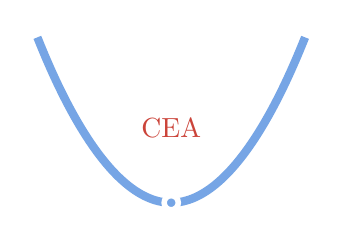
\begin{tikzpicture}
    % 1. Define the coordinates and font style
    \def\parabolapath{(-1.7, 1.15) parabola bend (0, -0.95) (1.7, 1.15)}

    % LAYER 1: Black Text
    \node[
        anchor=center,
        inner sep=0pt,
        font=\myfont,
        text=logoText
    ] at (0,0) {CEA};

    % LAYER 2: Parabola with a white outline
    \draw[white, line width=7pt] \parabolapath;
    \draw[logoParabola, line width=3pt] \parabolapath;

    % LAYER 3: Circle at the vertex
    \filldraw[fill=logoParabola, draw=white, line width=2pt] (0, -0.95) circle (0.09);

\end{tikzpicture}

\end{document}
